\chapter{Modélisation des véhicules}

Ce chapitre présente divers modèles cinématiques et dynamiques de véhicules qui sont souvent utilisés dans un contexte de commande et planification. C'est donc ici un survol d'approche de modélisation où un compromis entre fidélité et complexité est effectué. Les approches de modélisation haute fidélité qu'on pourrait utiliser dans un simulateur pour faire de la validation peuvent différer et ne seront pas traité ici.


\section{Navigation holonomique}

%%%%%%%%%%%%%%%%%%%%%%%%%
\begin{figure}[htbp]
	\centering
		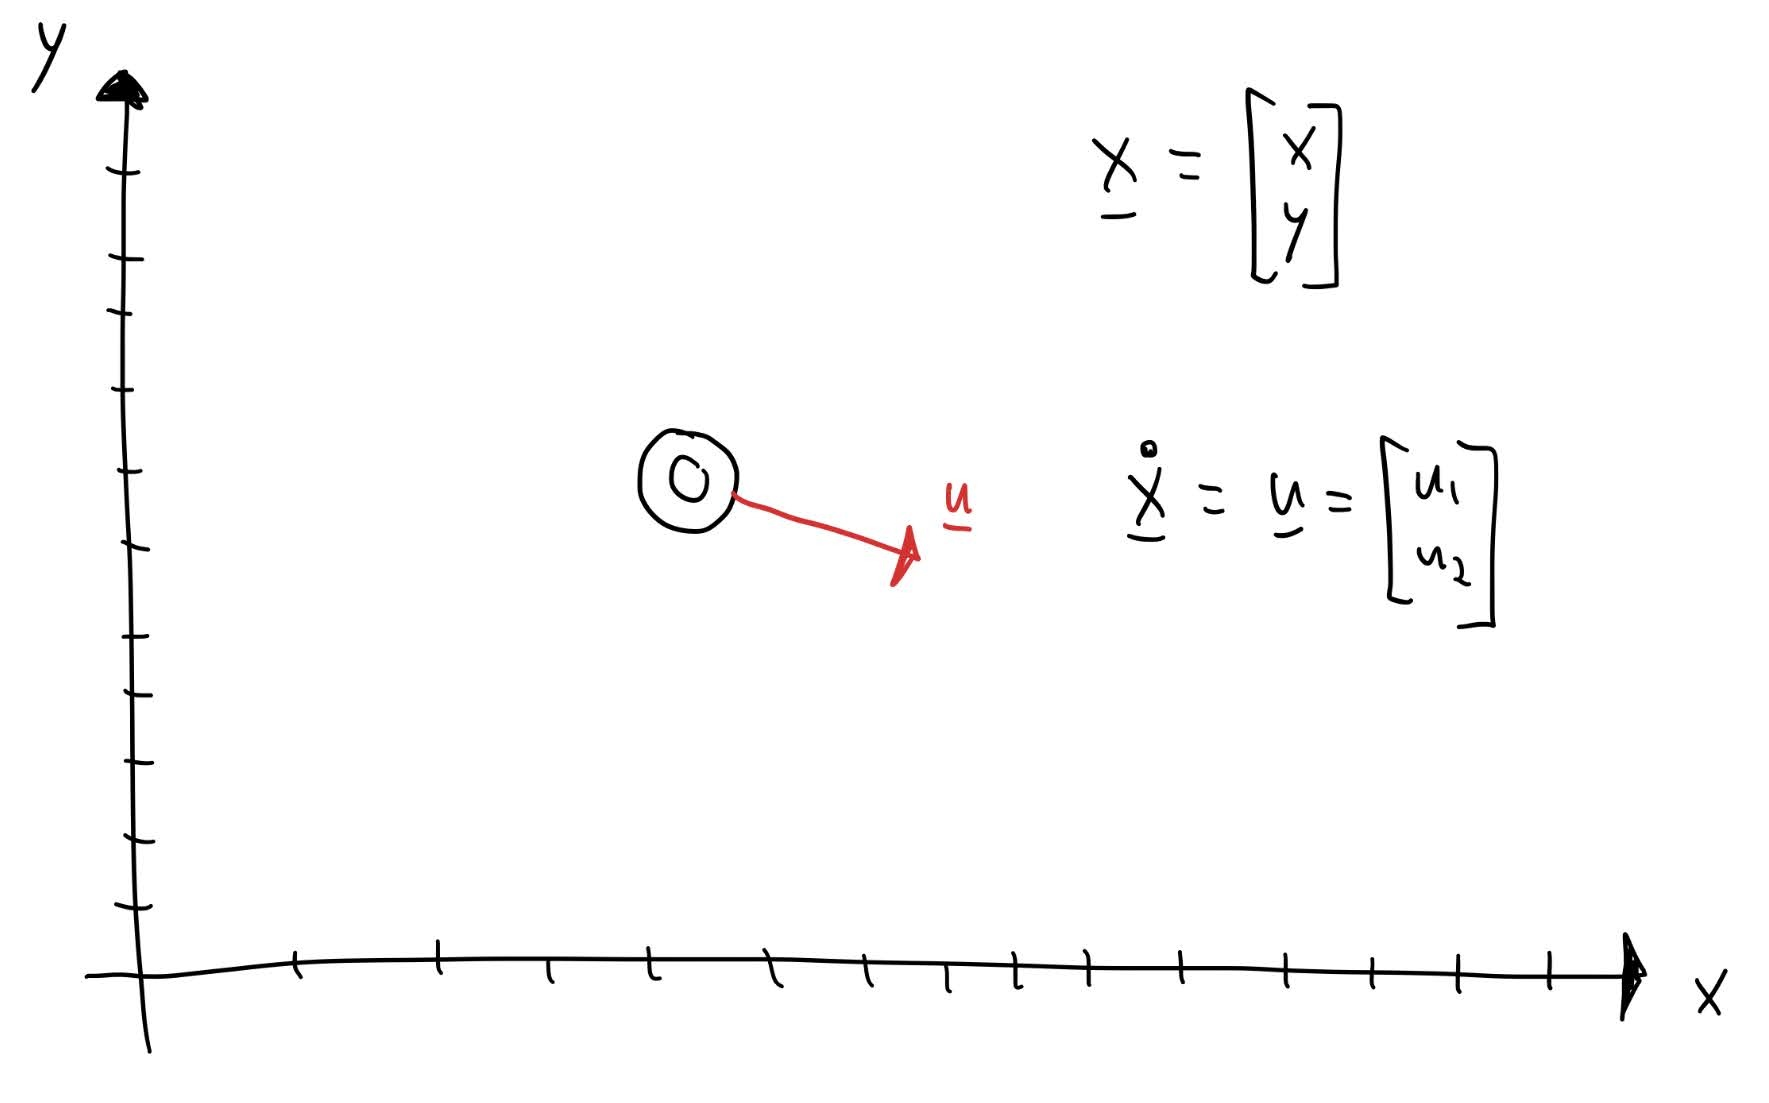
\includegraphics[width=0.70\textwidth]{fig/holonomicvehicle.jpg}
	\caption{Modèle dynamique pour un vehicle holonomique}
	\label{fig:holonomicvehicle}
\end{figure}
%%%%%%%%%%%%%%%%%%%%%%%%%


\section{Navigation sur un graphe discret}

À venir!



\section{Automobiles}

Cette section présente des modèles simples de comportement de véhicules qui ont une architecture de type automobile, c'est-à-dire quatre roue et des roues avant orientable (typiquement une architecture de direction de type ackerman).

%%%%%%%%%%%%%%%%%%%%%%%%%%%%%%%%%%%%%%%%
\subsection{Modèle bicyclette}

Le modèle souvent appelé bicyclette, est un modèle cinématique simple qui représente bien le comportement d'un véhicule a basse vitesse, et est donc typiquement utilisé pour planifié une trajectoire dans un stationnement par exemple.
%%%%%%%%%%%%%%%%%%%%%%%%%
\begin{figure}[htbp]
	\centering
		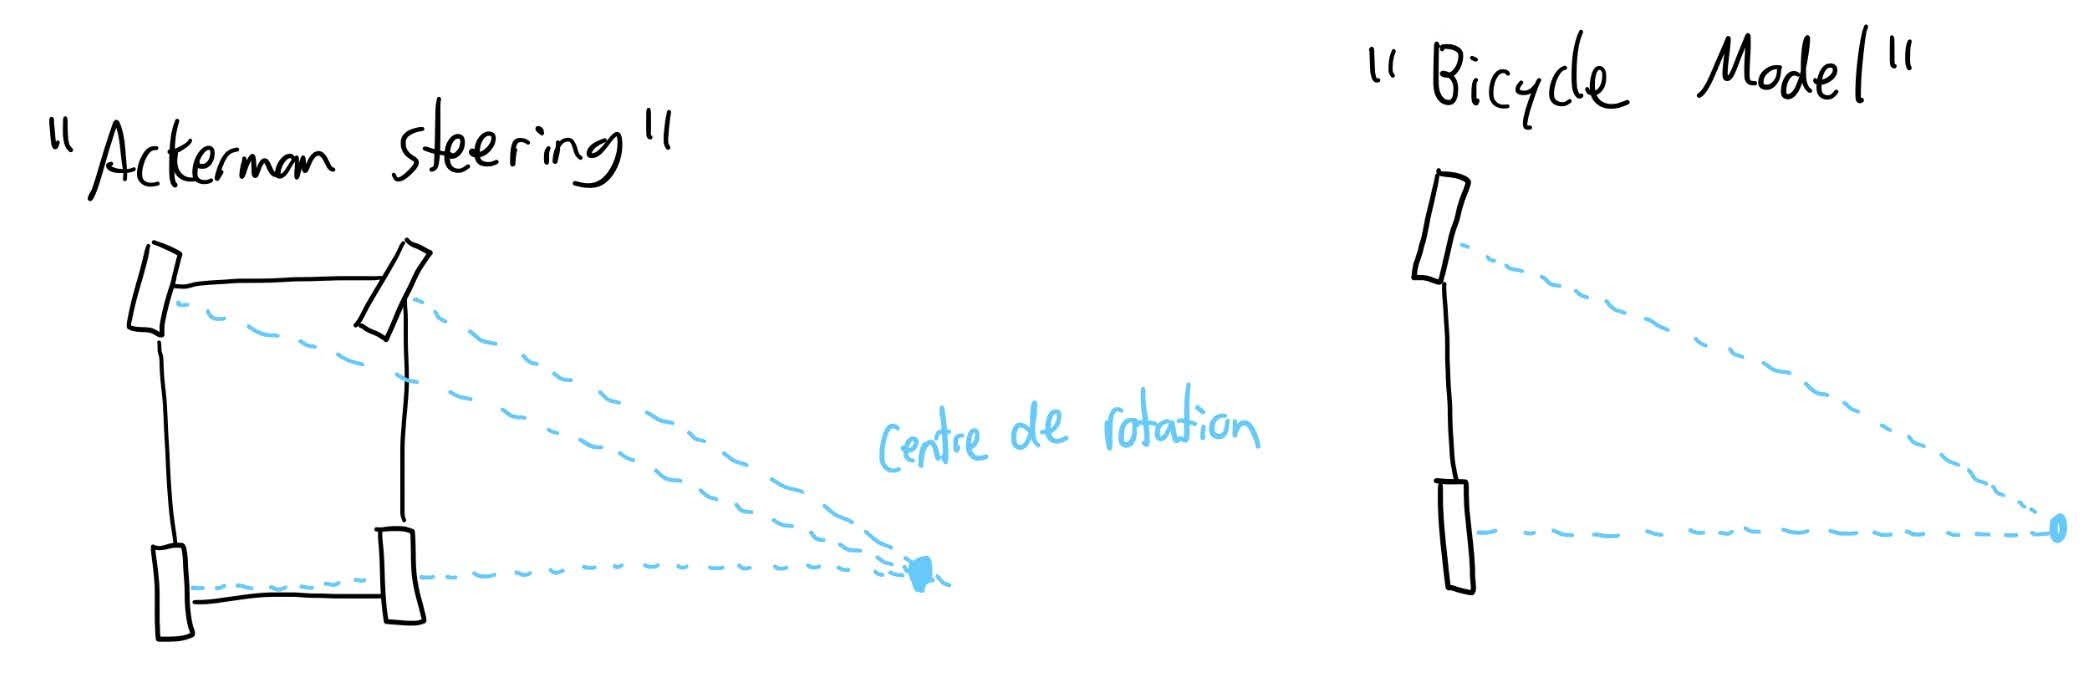
\includegraphics[width=0.90\textwidth]{fig/ackerman.jpg}
	\caption{Modèle simplifié de type bicyclette}
	\label{fig:ackerman}
\end{figure}
%%%%%%%%%%%%%%%%%%%%%%%%%

%%%%%%%%%%%%%%%%%%%%%%%%%%%%%%%%%%%%%%%%
\subsection{Modèle bicyclette cinématique}

%%%%%%%%%%%%%%%%%%%%%%%%%
\begin{figure}[htbp]
	\centering
		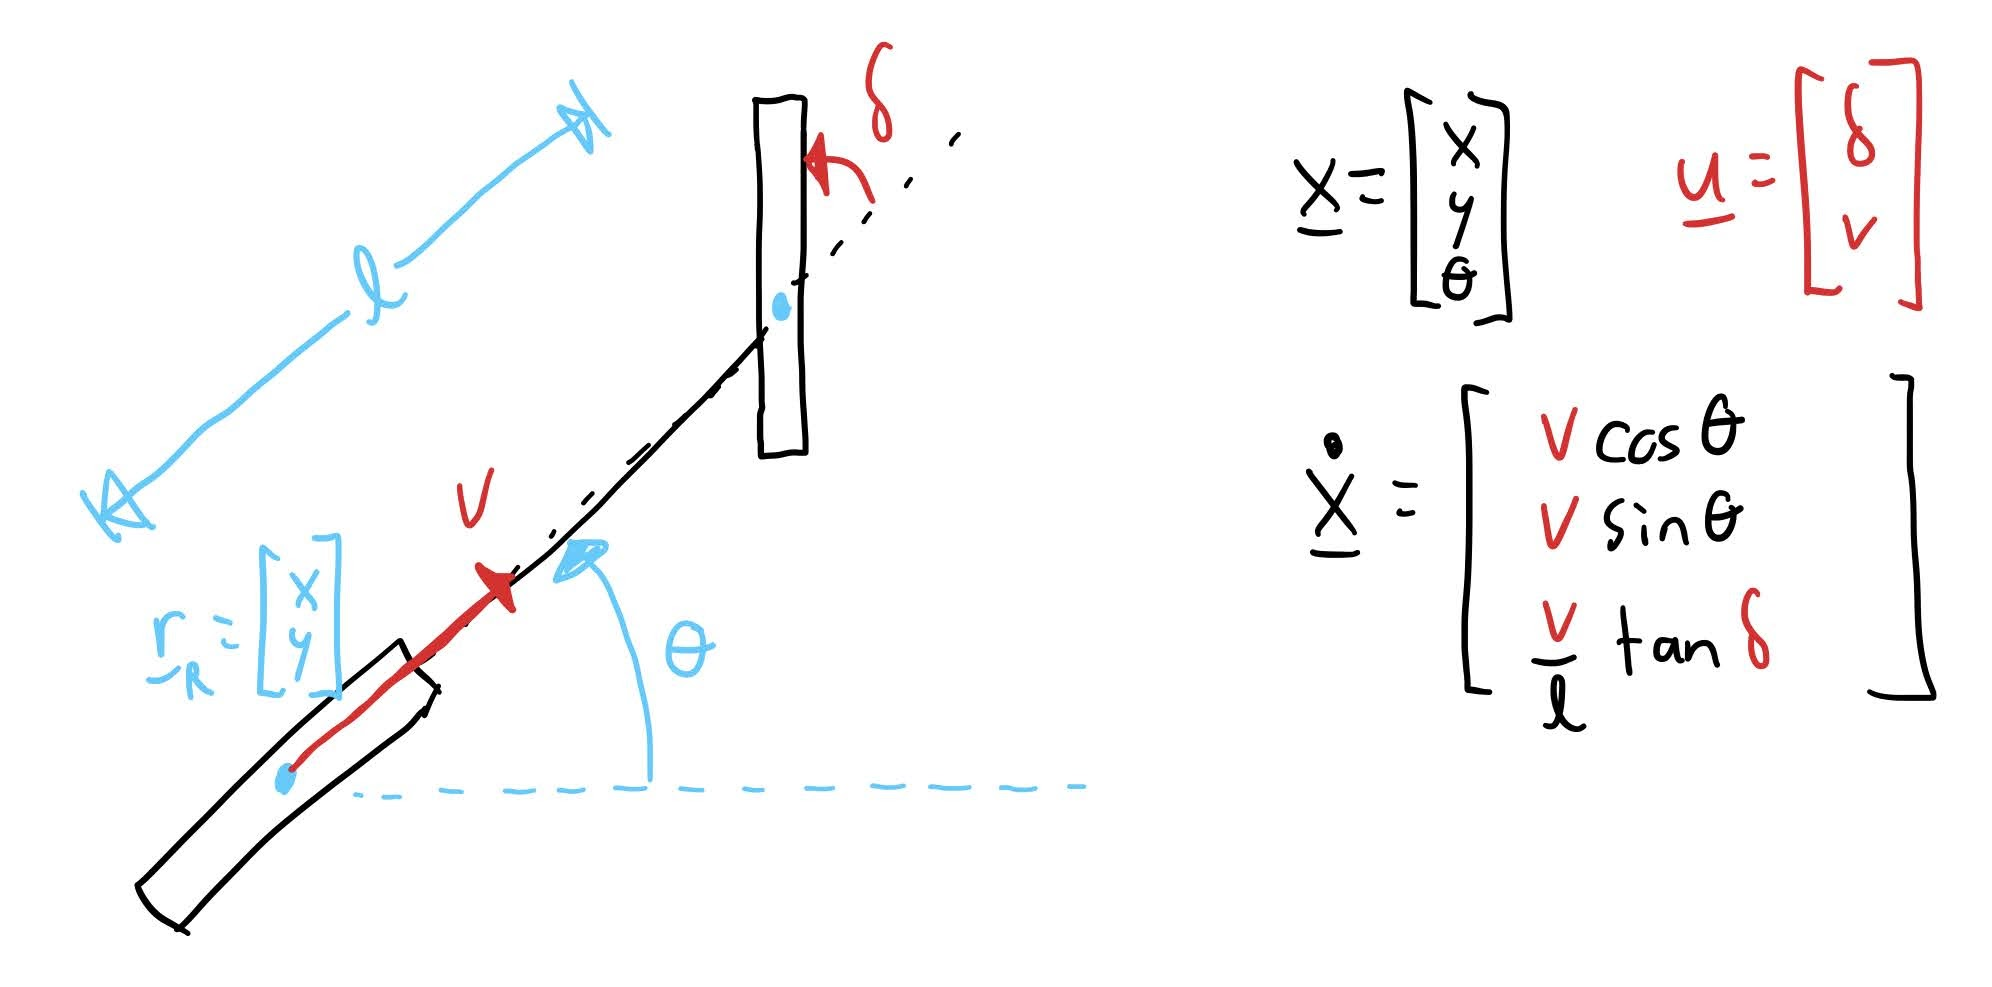
\includegraphics[width=0.90\textwidth]{fig/bicyclemodel.jpg}
	\caption{Modèle dynamique de type bicyclette cinématique}
	\label{fig:bicyclemodel}
\end{figure}
%%%%%%%%%%%%%%%%%%%%%%%%%

%%%%%%%%%%%%%%%%%%%%%%%%%
\begin{figure}[htbp]
	\centering
		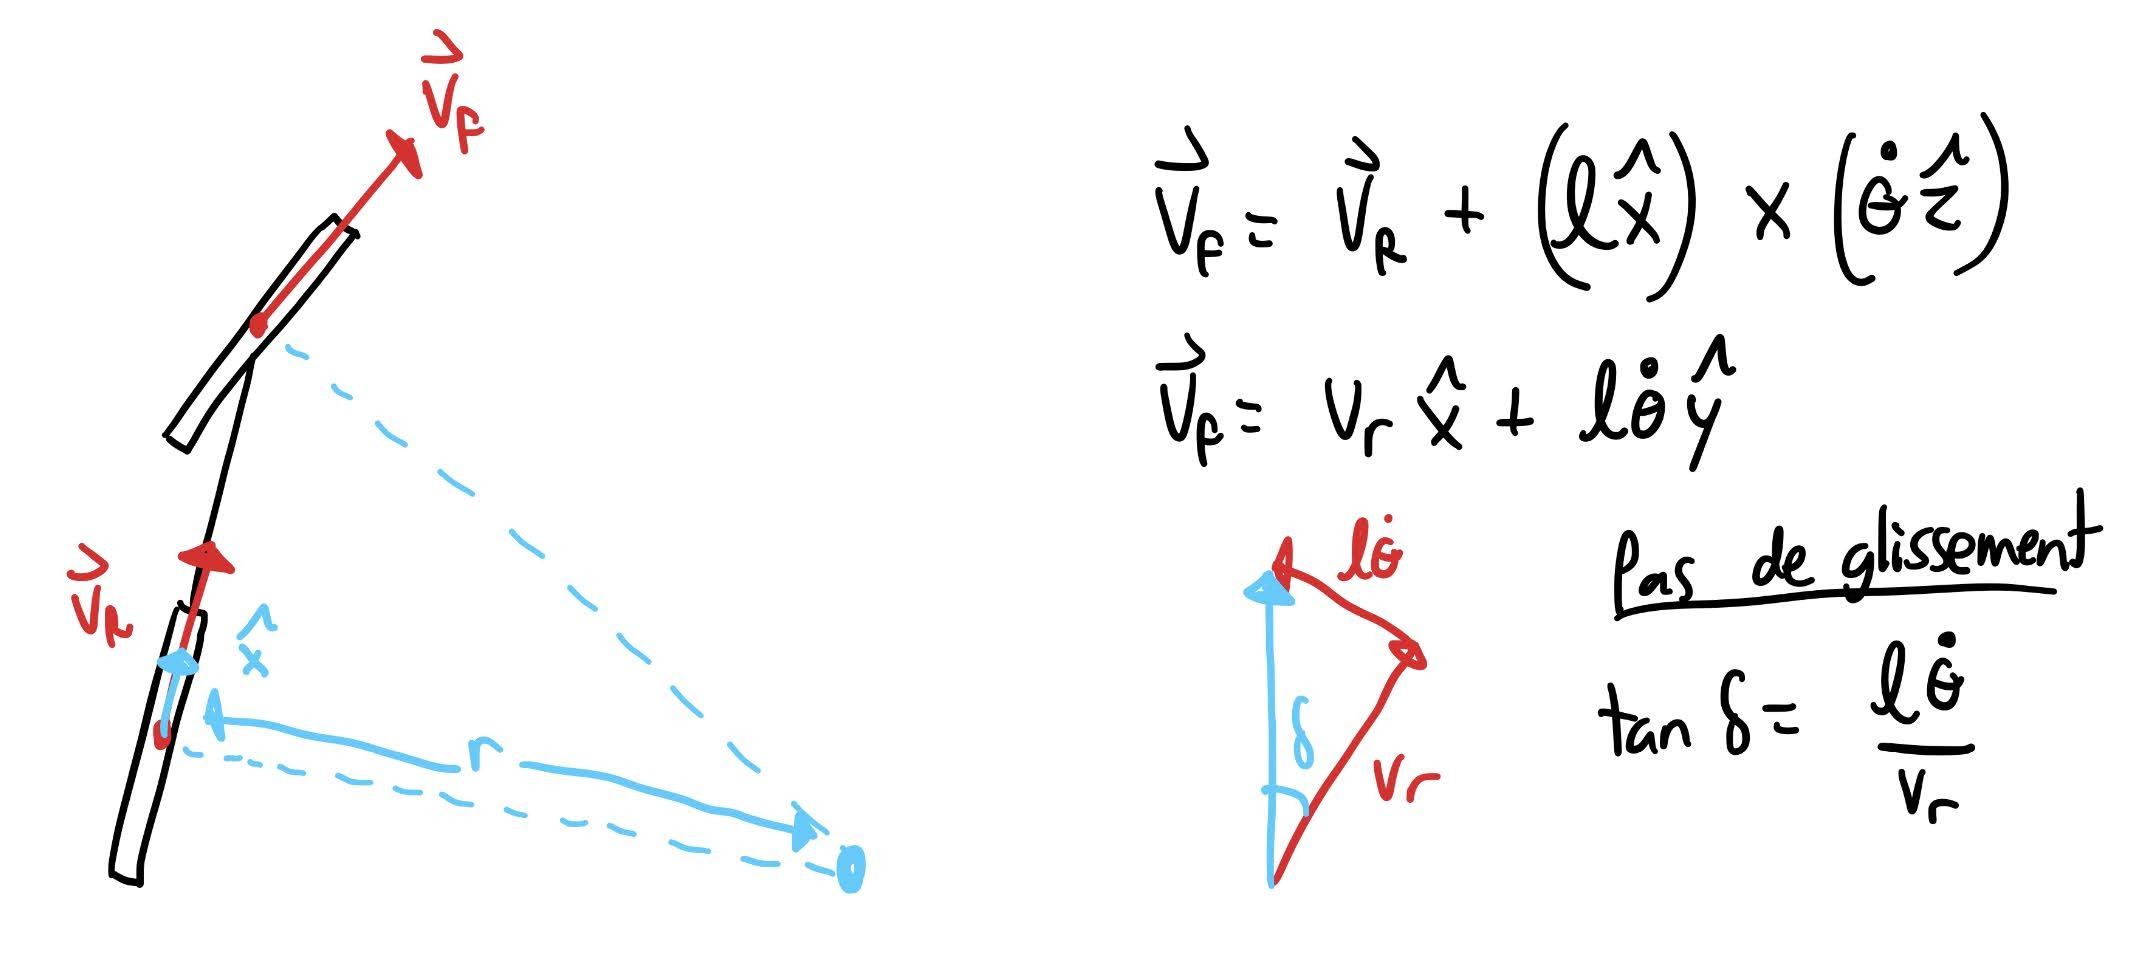
\includegraphics[width=0.90\textwidth]{fig/bicyclemodel2.jpg}
	\caption{Condition pour avoir aucun glissement pour le modèle bicyclette}
	\label{fig:bicyclemodel2}
\end{figure}
%%%%%%%%%%%%%%%%%%%%%%%%%

%%%%%%%%%%%%%%%%%%%%%%%%%%%%%%%%%%%%%%%%
\subsection{Modèle bicyclette dynamique}

À venir!


%%%%%%%%%%%%%%%%%%%%%%%%%%%%%%%%%%%%%%%%
\subsection{Modèle longitudinal}

%%%%%%%%%%%%%%%%%%%%%%%%%
\begin{figure}[htbp]
	\centering
		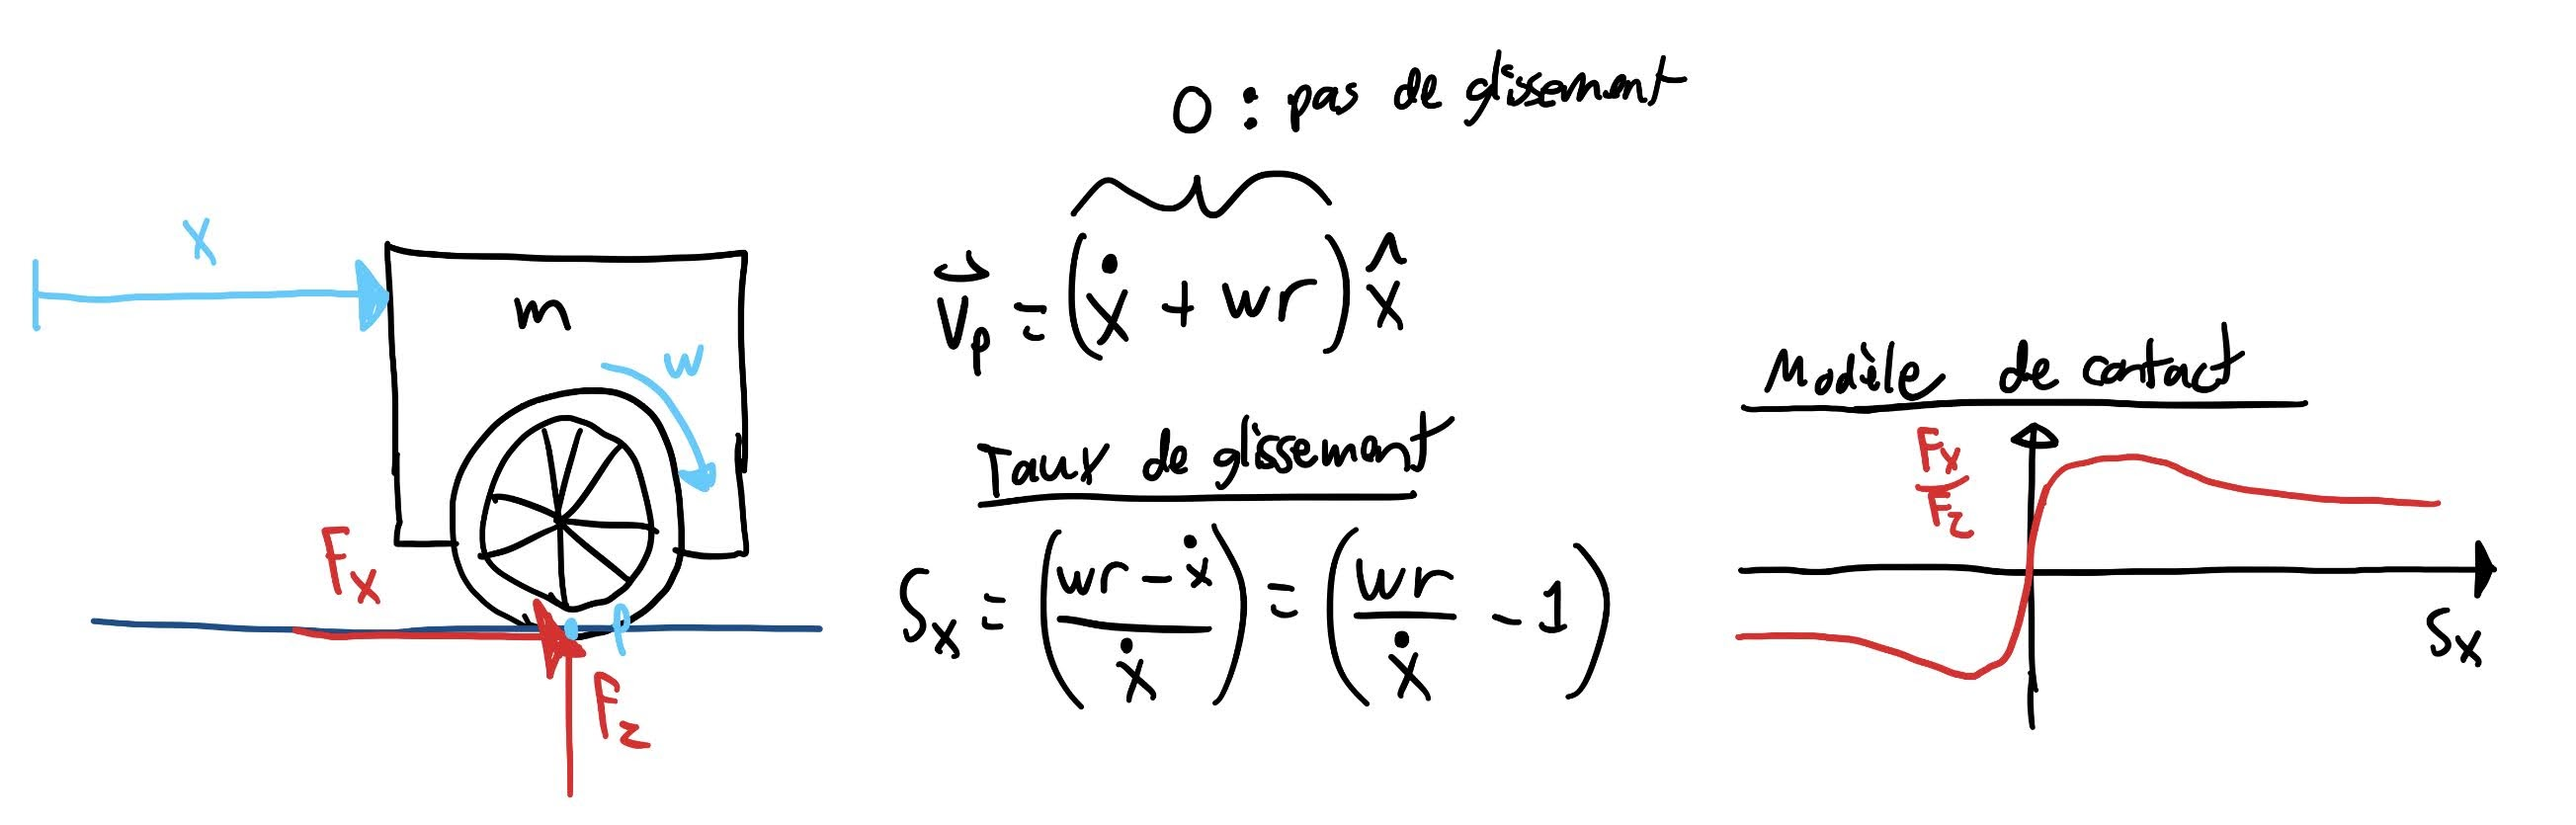
\includegraphics[width=0.90\textwidth]{fig/longitudinalmodel.jpg}
	\caption{Modèle simple de propulsion/freinage longitudinal}
	\label{fig:longitudinalmodel}
\end{figure}
%%%%%%%%%%%%%%%%%%%%%%%%%


\subsection{Modèle avec transfert de poids}


%%%%%%%%%%%%%%%%%%%%%%%%%%%%%%%%%%%%%%%%
\subsection{Modélisation du contact sol-roue}

%%%%%%%%%%%%%%%%%%%%%%%%%
\begin{figure}[htbp]
	\centering
		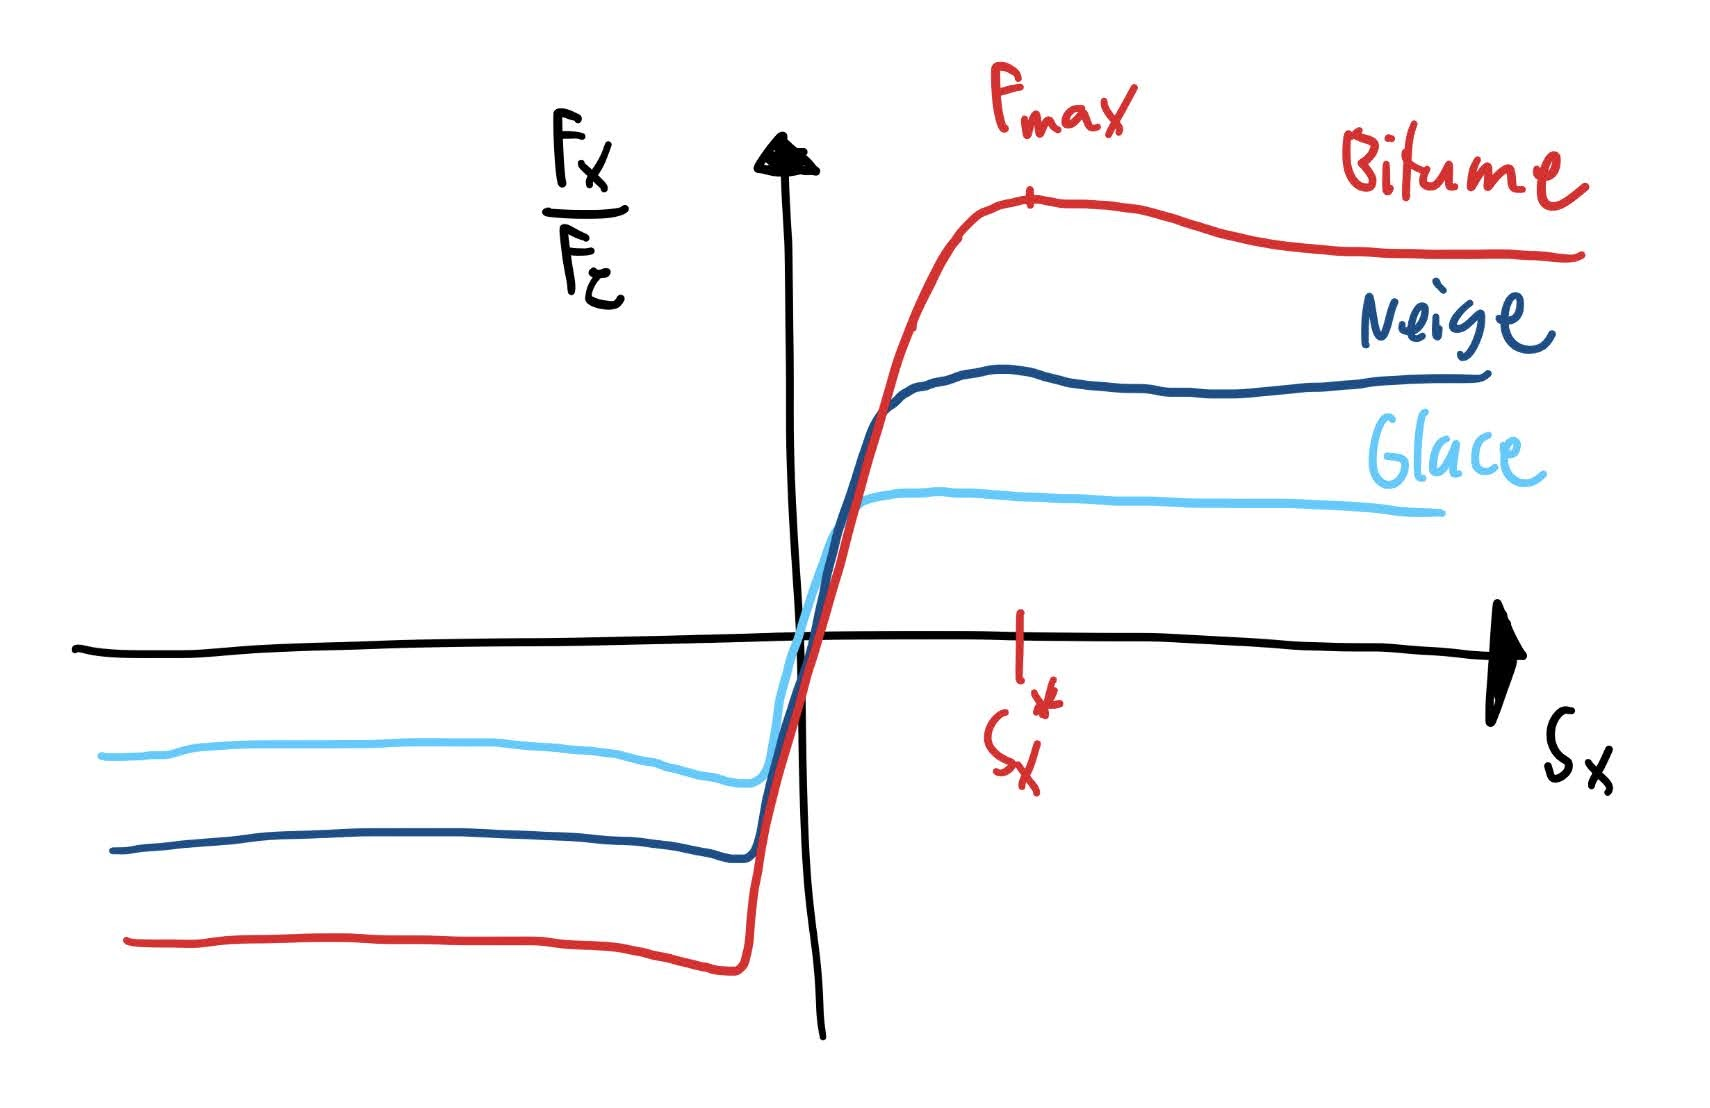
\includegraphics[width=0.60\textwidth]{fig/slipcurve.jpg}
	\caption{Modèle de force de contact pour un pneu}
	\label{fig:slipcurve}
\end{figure}
%%%%%%%%%%%%%%%%%%%%%%%%%





%%%%%%%%%%%%%%%%%%%%%%%%%%%%%%%%%%%%%%%%
\subsection{Modèles de suspension}

\subsubsection{Quart de véhicule sans pneu}

%%%%%%%%%%%%%%%%%%%%%%%%%
\begin{figure}[htbp]
	\centering
		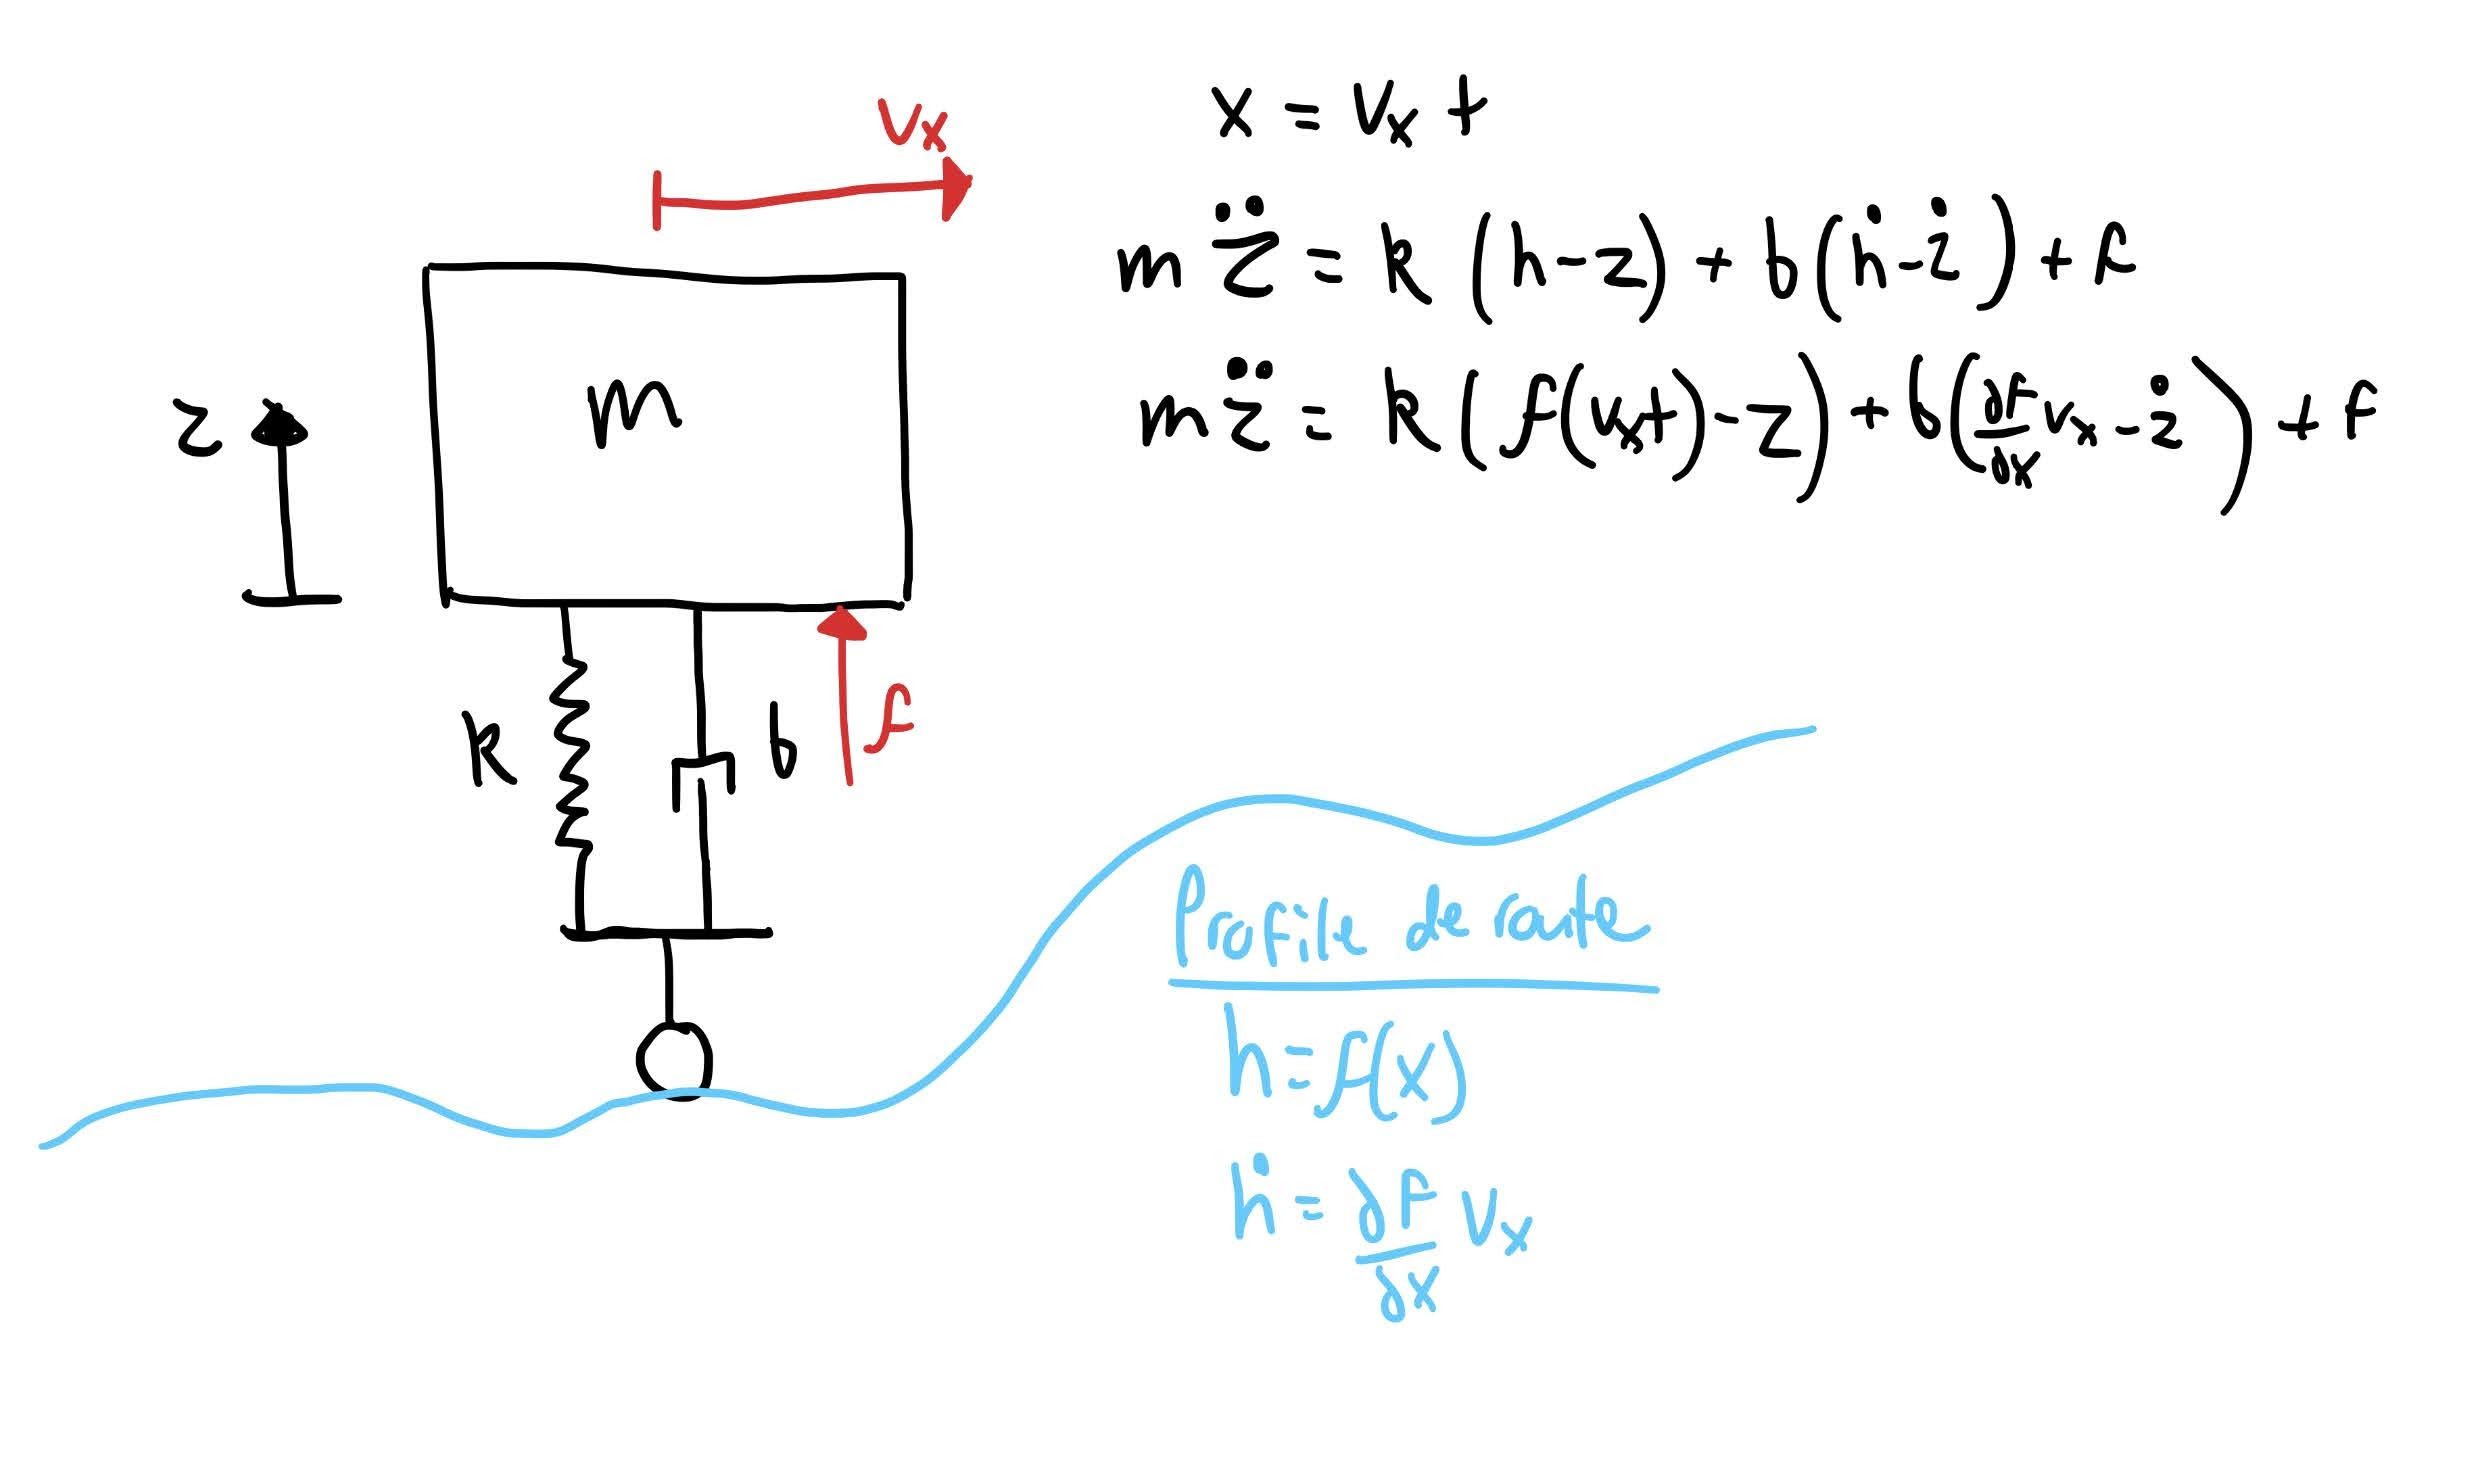
\includegraphics[width=0.90\textwidth]{fig/simplesuspension.jpg}
	\caption{Modèle simple de suspension}
	\label{fig:simplesuspension}
\end{figure}
%%%%%%%%%%%%%%%%%%%%%%%%%

\subsubsection{Quart de véhicule avec pneu}

\subsubsection{Demi véhicule}

\subsubsection{Véhicule complet}


\newpage
%%%%%%%%%%%%%%%%%%%%%%%%%%%%%%%%%%%%%%%%
\section{Robot mobiles}

Cette section présente des modèles simples pour d'autres architecture de robot mobiles.





\newpage
%%%%%%%%%%%%%%%%%%%%%%%%%%%%%%%%%%%%%%%%
\section{Drones}

\subsection{Modèle de quadrirotor planaire}

%%%%%%%%%%%%%%%%%%%%%%%%%
\begin{figure}[htbp]
	\centering
		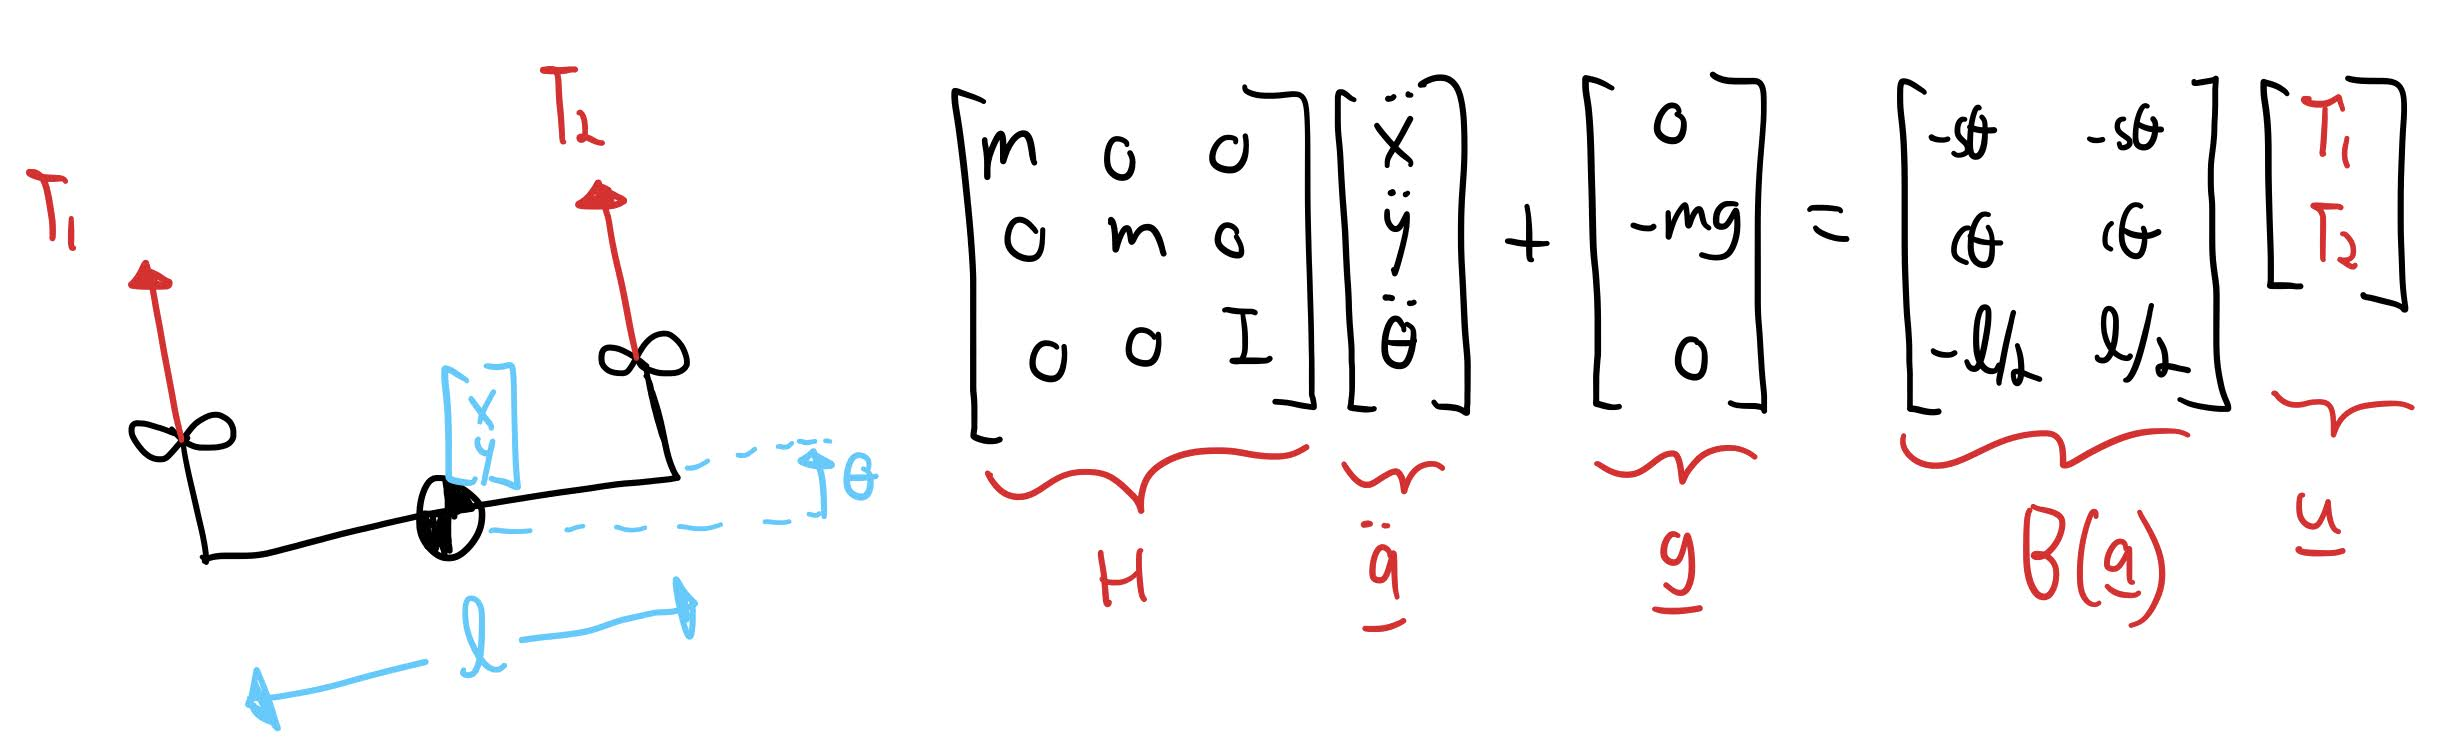
\includegraphics[width=0.99\textwidth]{fig/planar_drone.jpg}
	\caption{Modèle de drone planaire}
	\label{fig:planar_drone}
\end{figure}
%%%%%%%%%%%%%%%%%%%%%%%%%



\newpage
%%%%%%%%%%%%%%%%%%%%%%%%%%%%%%%%%%%%%%%%
\section{Avions}



\newpage
%%%%%%%%%%%%%%%%%%%%%%%%%%%%%%%%%%%%%%%%
\section{Fusée}